\newpage

\section{Additional Evaluation Results}\label{sec:evlaDetails}

Here we provide detailed results of time and memory consumption measurement for all queries.

\begin{figure}[h]
  \begin{center}
    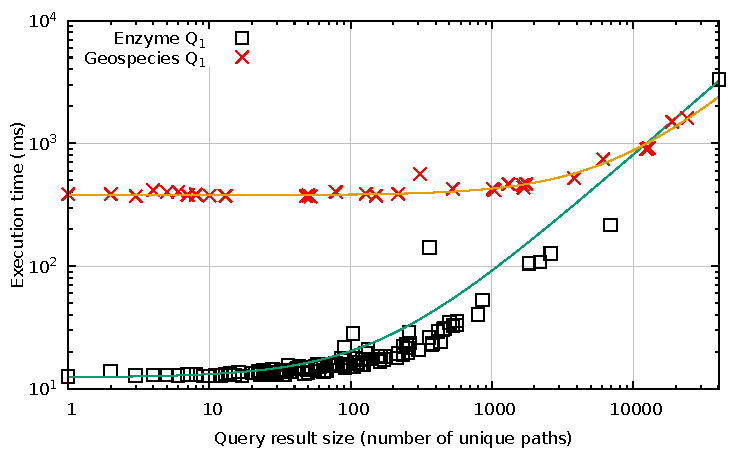
\includegraphics[width=0.5\textwidth]{data/time_per_paths_SCO.pdf}
    \caption{Execution time for $Q_1$ query}
    \label{fig:time_per_paths_SCO}
  \end{center}
\end{figure}


\begin{figure}[h]
  \begin{center}
    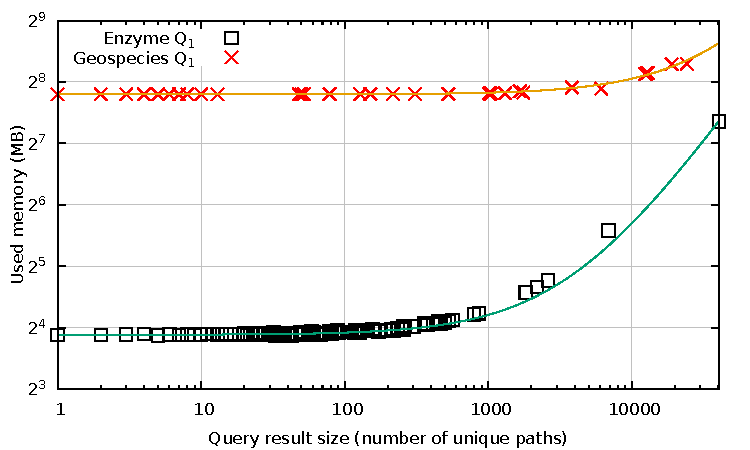
\includegraphics[width=0.5\textwidth]{data/mem_per_paths_SCO.pdf}
    \caption{Memory consumption for $Q_1$ query}
    \label{fig:mem_per_paths_SCO}
  \end{center}
\end{figure}


Time and memory measurements results for $Q_1$ query are provided in figures~\ref{fig:time_per_paths_SCO} and~\ref{fig:mem_per_paths_SCO} respectively.


\begin{figure}[h]
  \begin{center}
    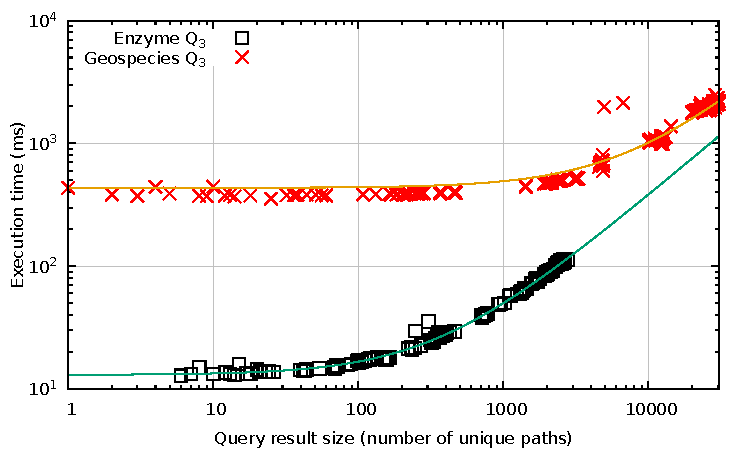
\includegraphics[width=0.5\textwidth]{data/time_per_paths_NT.pdf}
    \caption{Execution time for $Q_3$ query}
    \label{fig:time_per_paths_NT}
  \end{center}
\end{figure}

\begin{figure}[h]
  \begin{center}
    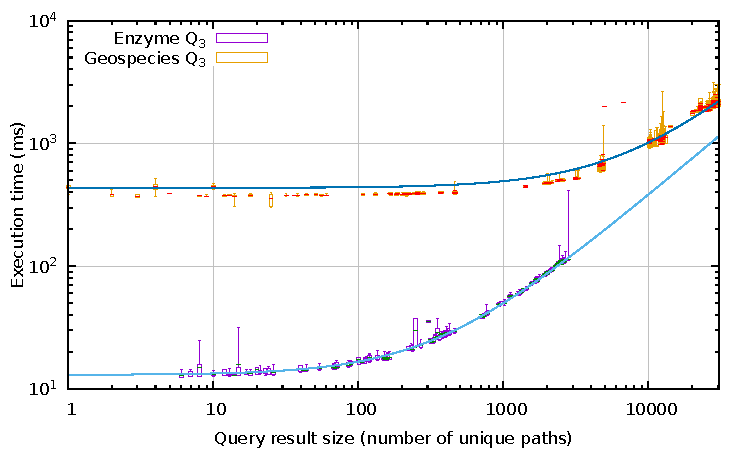
\includegraphics[width=0.5\textwidth]{data/time_per_paths_NT_boxplot.pdf}
    \caption{Execution time for $Q_3$ query (boxplot)}
    \label{fig:time_per_paths_NT_boxplot}
  \end{center}
\end{figure}


Time measuremet results for $Q_3$ query are provided in two ways: only average values for each query result size (figure~\ref{fig:time_per_paths_NT}) and standard boxplot to provide information about vales distribution (figure~\ref{fig:time_per_paths_NT_boxplot}). We can see that number of outliers is small. Note that the number of measurements for each query result size is different, so in some cases we have jus single points instead of boxes (it means that there is only one result of such size).


\begin{figure}[h]
  \begin{center}
    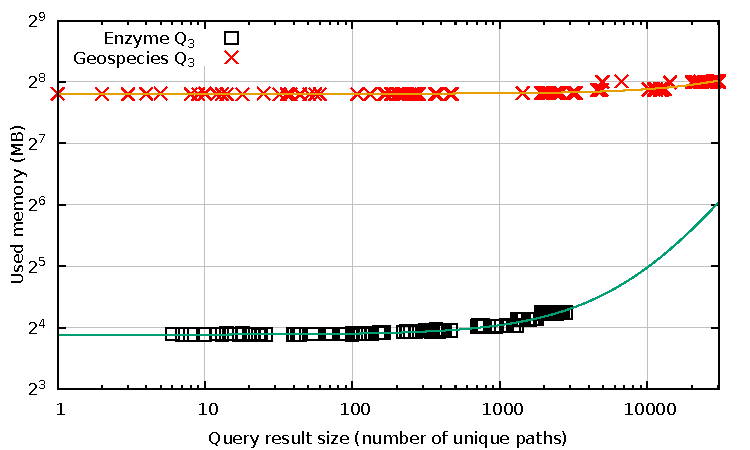
\includegraphics[width=0.5\textwidth]{data/mem_per_paths_NT.pdf}
    \caption{Memory consumption for $Q_3$ query}
    \label{fig:mem_per_paths_NT}
  \end{center}
\end{figure}

Memory consumption for $Q_3$ query is presented in figure~\ref{fig:mem_per_paths_NT}.

Also we can see, that for provided queries and graphs time and memory consumption are not depend on query: for similar result sizes reqired time and memory are similar for all qieryes.